\section{Thiết lập thực nghiệm}
\label{sec:experiments}

\subsection{Bộ dữ liệu chuẩn Refined Deep-SAR Oil Spill (SOS)}
\label{subsec:dataset}
Nghiên cứu sử dụng bộ dữ liệu công khai Deep-SAR Oil Spill (SOS), được giới thiệu bởi Zhu và cộng sự~\cite{zhu2022oil} và chuẩn hóa trên kho lưu trữ Zenodo~\cite{zuenko2025refined}. Bộ dữ liệu được xây dựng từ 21 cảnh ảnh vệ tinh SAR thô bao phủ hai khu vực xảy ra thảm họa tràn dầu lớn:
\begin{enumerate}
    \item \textbf{Vịnh Mexico (Sự cố tràn dầu Deepwater Horizon, năm 2010):} Bao gồm 14 cảnh ảnh thu nhận từ cảm biến ALOS PALSAR băng L (sản phẩm mức 1.5), độ phân giải lấy mẫu không gian $12.5\text{ m}$, kênh phân cực ngang-ngang (HH).
    \item \textbf{Vịnh Ba Tư (Khu vực mỏ dầu Al-Khafji, năm 2017):} Bao gồm 7 cảnh ảnh thu nhận từ cảm biến Sentinel-1A băng C ở chế độ quét rộng giao thoa (IW) mức 1 (GRD), độ phân giải không gian $5\text{ m} \times 20\text{ m}$, góc tới dao động từ $29.1^\circ$ đến $46^\circ$, kênh phân cực dọc-dọc (VV).
\end{enumerate}

\begin{table}[!t]
\centering
\caption{Thống kê cấu trúc phân chia bộ dữ liệu Refined Deep-SAR Oil Spill (SOS).}
\label{tab:dataset_stats}
\resizebox{\linewidth}{!}{%
\begin{tabular}{lcc}
\toprule
\textbf{Thuộc tính} & \textbf{Sentinel-1A (Vịnh Ba Tư)} & \textbf{ALOS PALSAR (Vịnh Mexico)} \\
\midrule
Cảm biến vệ tinh & Sentinel-1A & ALOS PALSAR \\
Băng tần radar & Băng C ($\sim 5.6\text{ cm}$) & Băng L ($\sim 23.6\text{ cm}$) \\
Kênh phân cực & VV & HH \\
Độ phân giải danh định & $5\text{ m} \times 20\text{ m}$ & $12.5\text{ m}$ \\
Sự cố tràn dầu & Al-Khafji (2017) & Deepwater Horizon (2010) \\
Số cảnh ảnh thô gốc & 7 cảnh & 14 cảnh \\
Kích thước patch chuẩn hóa & $256 \times 256$ pixels & $256 \times 256$ pixels \\
\midrule
Tập huấn luyện (Train) & $2\,683$ ảnh & Không sử dụng ($3\,101$ ảnh lưu kho) \\
Tập kiểm định (Validation) & $671$ ảnh & Không sử dụng \\
Tập kiểm thử (Test độc lập) & $839$ ảnh (thư mục \texttt{val} gốc) & $776$ ảnh (Test ngoài cảm biến, \texttt{val} gốc) \\
\midrule
\textbf{Tổng số mẫu ảnh sử dụng} & \textbf{4\,193 ảnh} & \textbf{776 ảnh} \\
\bottomrule
\end{tabular}%
}
\end{table}

\noindent\textbf{Giao thức phân chia dữ liệu và giới hạn cấp cảnh:}
Theo nhà phát hành bộ dữ liệu~\cite{zuenko2025refined}, 21 cảnh SAR gốc được cắt thành các mảnh nhỏ, tăng cường dữ liệu và chuẩn hóa về kích thước $256 \times 256$ pixels. Để đảm bảo tính liêm chính thực nghiệm, chúng tôi thiết lập giao thức phân chia 3 tập nghiêm ngặt (Bảng~\ref{tab:dataset_stats}):
\begin{itemize}
    \item $3\,354$ ảnh của tập huấn luyện gốc Sentinel-1A (\texttt{train/}) được phân chia theo tỷ lệ 80:20 (phân tầng theo ảnh rỗng và có dầu với seed $2026$) thành: \textbf{2\,683 ảnh Train} (dùng để trích xuất mẫu huấn luyện SVM/CART) và \textbf{671 ảnh Validation} (dùng độc quyền để sàng lọc 110 cấu hình lọc/ngưỡng và 729 cấu hình mô hình vùng).
    \item $839$ ảnh của phân tập kiểm định gốc Sentinel-1A (\texttt{val/} của nhà phát hành) được giữ nguyên làm \textbf{tập Test độc lập}, chỉ được mở khóa đánh giá một lần duy nhất cho cấu hình chiến thắng sau khi toàn bộ quy trình và mô hình đã được đóng băng.
    \item $776$ ảnh của phân tập \texttt{val/} gốc thuộc ALOS PALSAR được sử dụng làm \textbf{tập kiểm thử ngoài cảm biến} (out-of-sensor test) với mô hình đã đóng băng từ Sentinel-1A (không sử dụng $3\,101$ ảnh \texttt{train/} của PALSAR).
\end{itemize}
Cần lưu ý một giới hạn thực nghiệm quan trọng: do bộ dữ liệu công khai trên Zenodo không kèm định danh cảnh gốc (scene ID) hay tọa độ địa lý, việc phân chia được thực hiện ở cấp patch, do đó không thể bảo đảm tính độc lập tuyệt đối theo cảnh thô viễn thám ban đầu.

\noindent\textbf{Không gian tìm kiếm siêu tham số $110 \times 729$ và quy tắc lựa chọn:}
Quá trình lựa chọn mô hình trên $671$ ảnh Validation được tiến hành theo hai bước có kiểm soát:
\begin{enumerate}
    \item \textit{Sàng lọc bộ lọc và ngưỡng tạo ứng viên (110 cấu hình, cố định hình thái học \texttt{none} và $A_{\min} = 16$):} Kết hợp tích Đề-các giữa \textbf{11 bộ lọc} (\texttt{none}; \texttt{median} kích thước $\{3, 5\}$; \texttt{gaussian} với $\sigma \in \{0.8, 1.2\}$; \texttt{lee} với kích thước $\{3, 5, 7\} \times L \in \{1, 4\}$) và \textbf{10 bộ phân ngưỡng} (\texttt{otsu} toàn cục; \texttt{niblack} cục bộ với cửa sổ $\{15, 31, 51\} \times k \in \{0.2, 0.5, 0.8\}$).
    \item \textit{Tìm kiếm cấu hình hình thái, đặc trưng và bộ phân loại (729 cấu hình):} Giữ lại Top-3 cấu hình lọc/ngưỡng đầu bảng (Lee $7\times 7, L=4$ + Otsu; Lee $7\times 7, L=1$ + Otsu; Lee $5\times 5, L=4$ + Otsu) và quét toàn diện tích Đề-các: $3 \text{ (cấu hình lọc/ngưỡng)} \times 3 \text{ (phép hình thái $3\times 3$: \texttt{none, close, open\_close})} \times 3 \text{ (ngưỡng diện tích } A_{\min} \in \{4, 16, 64\}) \times 3 \text{ (nhóm đặc trưng: \texttt{shape, intensity, all})} \times 9 \text{ (mô hình: 6 cấu hình CART với } \text{max\_depth} \in \{3, 5, 8\} \times \text{min\_leaf} \in \{5, 20\} \text{ và 3 cấu hình LinearSVM với } C \in \{0.1, 1, 10\}) = 729$ tổ hợp.
    \item \textit{Quy tắc xếp hạng và thiên lệch lựa chọn:} Tại mỗi bước, các cấu hình nằm trong dải $\text{F1-band} = 0.005$ so với mức F1 cao nhất được ưu tiên xếp hạng theo độ thu hồi Recall giảm dần, sau đó theo thời gian chạy tăng dần. Việc chọn cấu hình đứng đầu từ 729 tổ hợp trên cùng tập Validation (671 ảnh) tất yếu mang lại một mức độ lạc quan do lựa chọn (selection optimism) đối với các con số trên Validation, do đó hiệu năng thực tế phải được phán quyết trên tập Test độc lập ($839$ ảnh).
\end{enumerate}

Mặt nạ nhị phân ground truth $G \in \{0, 1\}^{H \times W}$ được xác lập bằng ngưỡng chuẩn:
\begin{equation}
G(x, y) = [M_{\text{raw}}(x, y) \ge 128]
\end{equation}

\subsection{Giao thức phân tầng theo tỷ lệ diện tích dầu}
\label{subsec:regimes}
Dựa trên tỷ lệ diện tích dầu $r = \frac{1}{HW}\sum_{x, y} G(x, y)$, toàn bộ dữ liệu được phân tầng thành 5 chế độ diện tích:
\begin{itemize}
    \item \textbf{$R_0$ (Biển sạch):} $r = 0$, khung cảnh không chứa dầu, kiểm định tỷ lệ cảnh báo sai (False Alarm).
    \item \textbf{$R_1$ (Vết dầu nhỏ):} $0 < r < 0.05$, diện tích dầu dưới 5\% khung ảnh, mô phỏng các vết dầu mới rò rỉ.
    \item \textbf{$R_2$ (Vết dầu trung bình):} $0.05 \le r < 0.50$, bao gồm các dải dầu dài, hẹp hoặc bị phân mảnh.
    \item \textbf{$R_3$ (Vết dầu diện rộng):} $0.50 \le r < 0.95$, vệt dầu bao phủ phần lớn khung ảnh.
    \item \textbf{$R_4$ (Patch ngập dầu toàn phần):} $0.95 \le r \le 1.00$, khung ảnh nằm trọn trong vệt dầu lớn.
\end{itemize}

\begin{table}[!t]
\centering
\caption{Phân bố số lượng ảnh thực tế theo 5 chế độ diện tích ($R_0 \to R_4$) trên tập kiểm thử độc lập Sentinel-1A (839 ảnh) và tập kiểm thử ngoài cảm biến ALOS PALSAR (776 ảnh).}
\label{tab:regime_counts}
\resizebox{\linewidth}{!}{%
\begin{tabular}{lccccc}
\toprule
\textbf{Tập kiểm thử} & \textbf{$R_0$} & \textbf{$R_1$} & \textbf{$R_2$} & \textbf{$R_3$} & \textbf{$R_4$} \\
\midrule
Sentinel-1A Test (839 ảnh, \texttt{val/} gốc) & 31 & 99 & 457 & 196 & 56 \\
ALOS PALSAR Test ngoài cảm biến (776 ảnh, \texttt{val/} gốc) & 45 & 113 & 585 & 31 & 2 \\
\bottomrule
\end{tabular}%
}
\end{table}

\begin{figure*}[!t]
\centering
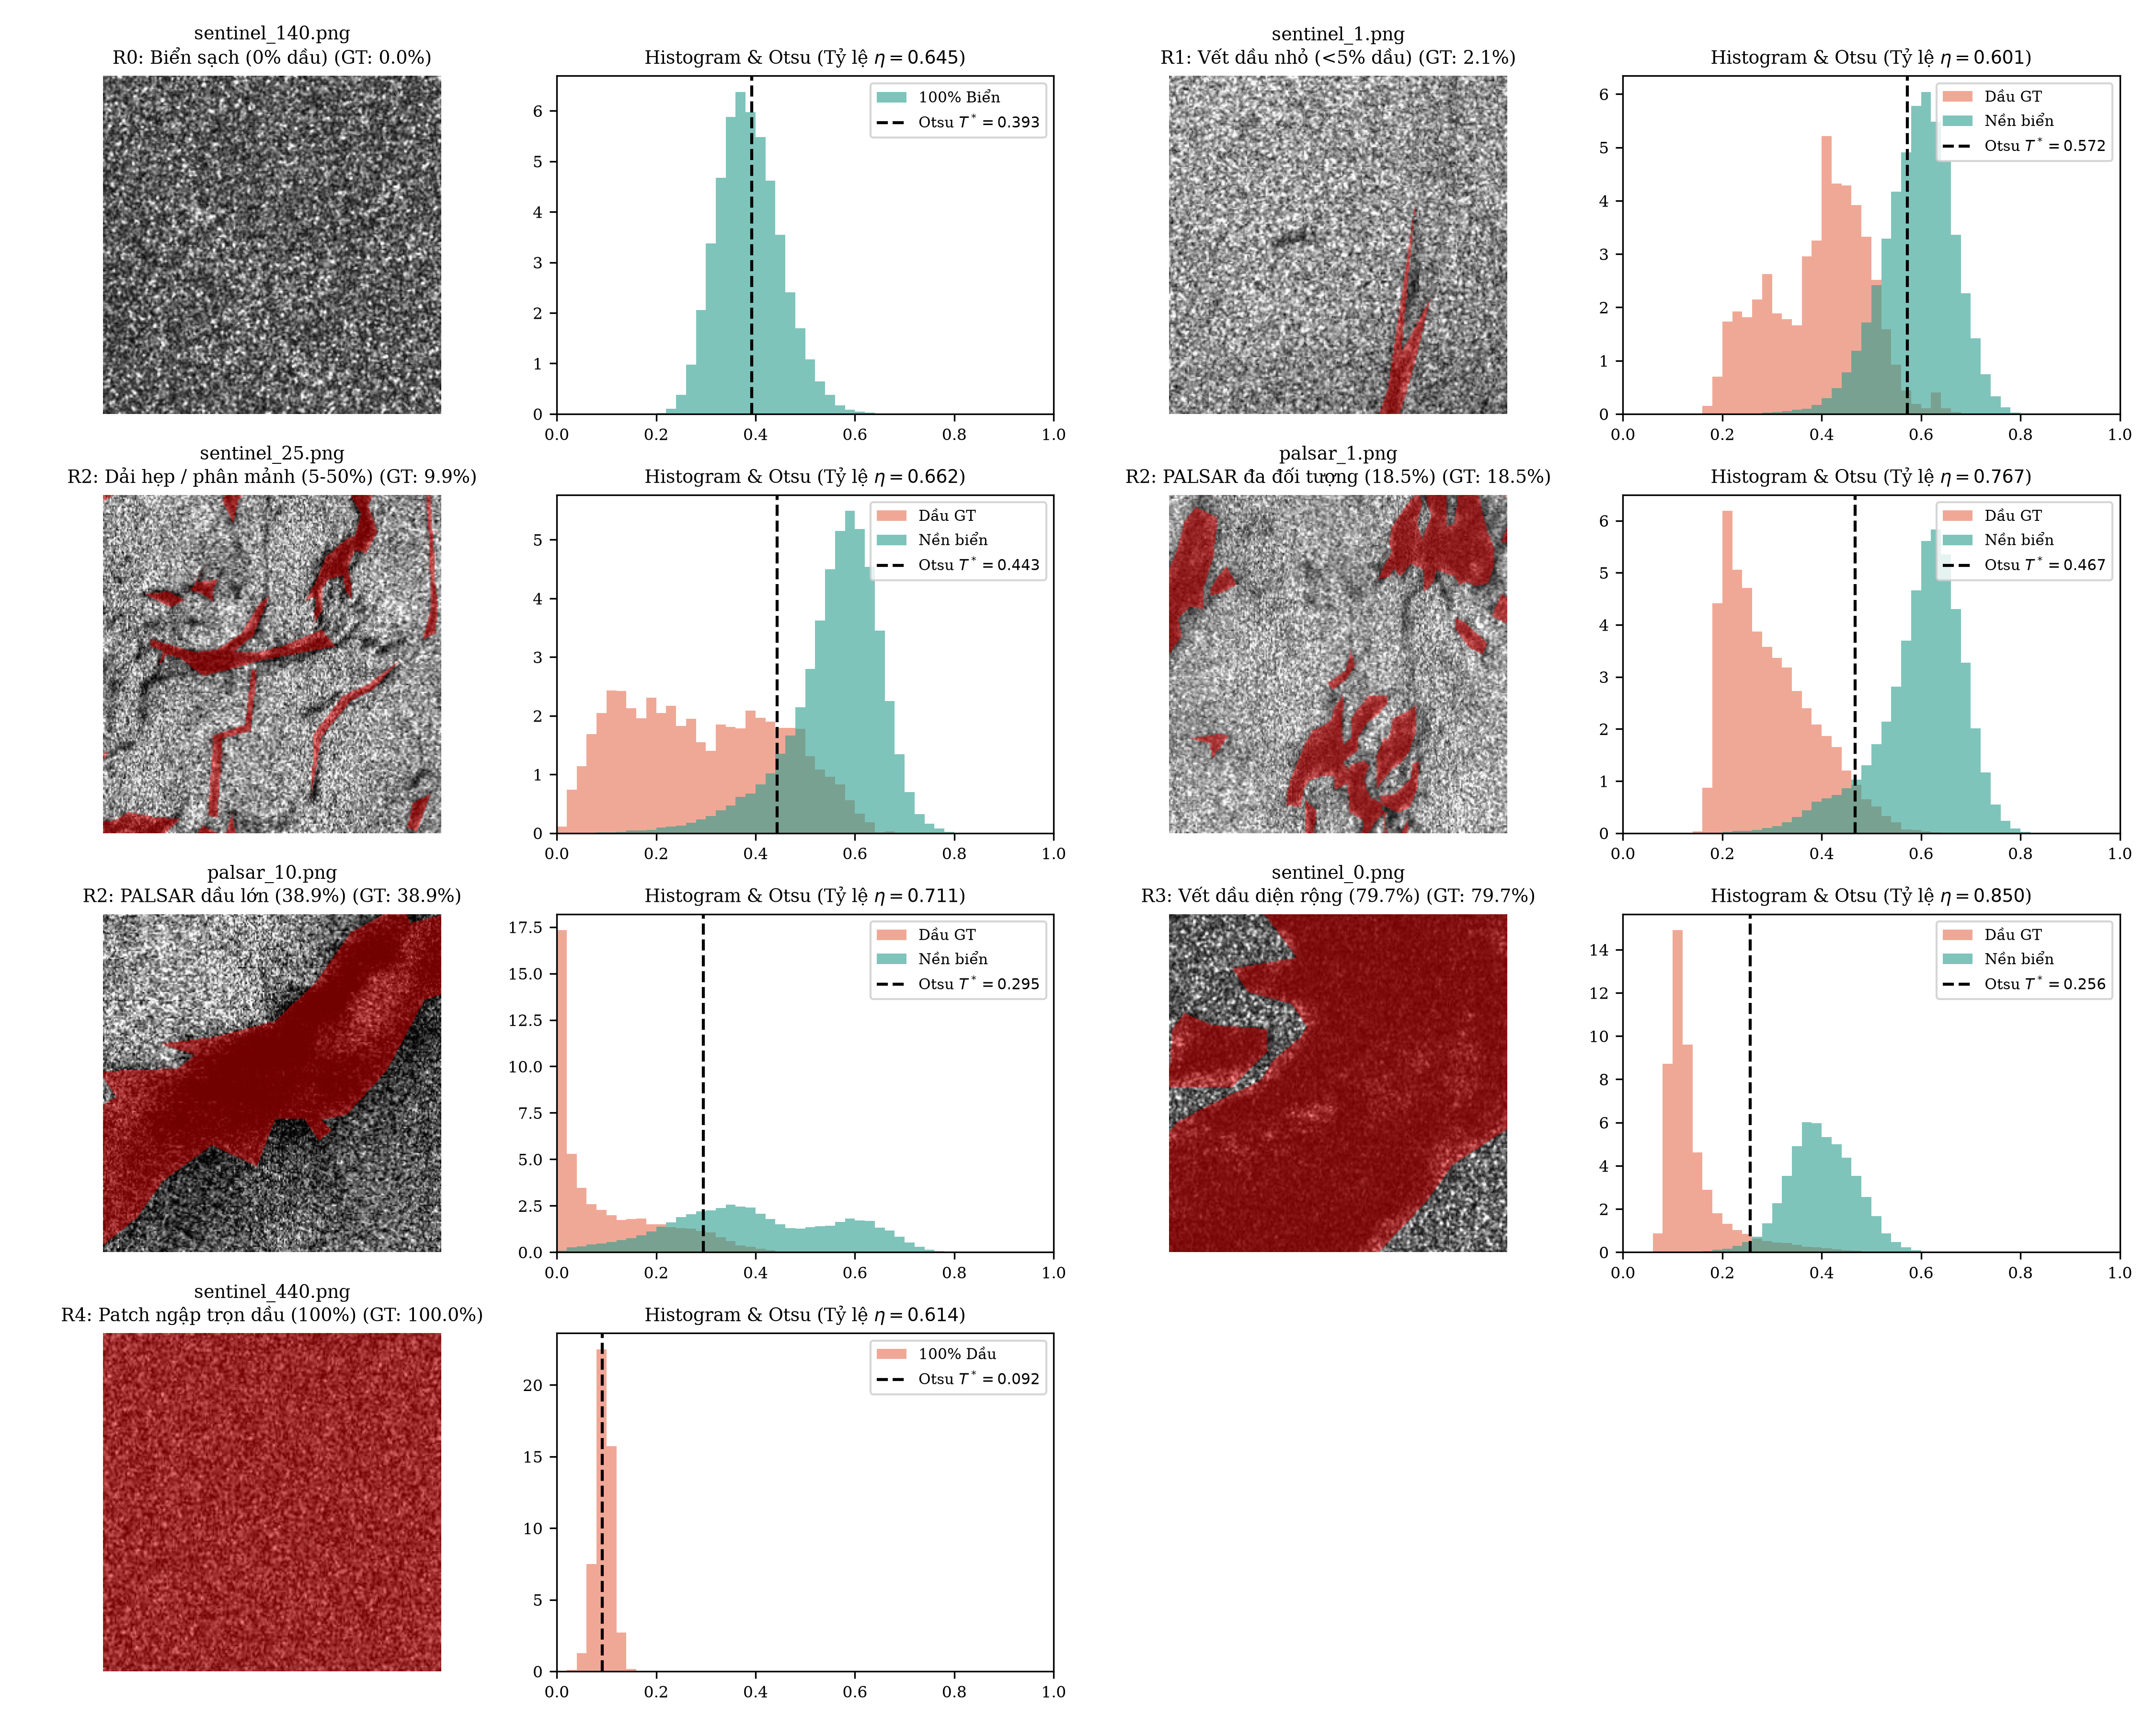
\includegraphics[width=\textwidth]{figures/fig2_sos_dataset_regimes.png}
\caption{Minh họa các mẫu ảnh SAR thực tế, mặt nạ Ground Truth và phân bố Histogram kèm ngưỡng Otsu $T^*$ và tỷ số phương sai $\eta = \sigma_B^2(T^*)/\sigma_T^2$ qua 5 chế độ diện tích dầu ($R_0 \to R_4$). Nguồn ảnh trích từ phân tập \texttt{val/} gốc của nhà phát hành SOS (tương ứng tập Test độc lập, chỉ dùng để minh họa định tính sau khi đã đóng băng mô hình): \texttt{sentinel\_140.png} ($R_0$), \texttt{sentinel\_1.png} ($R_1$), \texttt{sentinel\_25.png}, \texttt{palsar\_1.png}, \texttt{palsar\_10.png} ($R_2$), \texttt{sentinel\_0.png} ($R_3$) và \texttt{sentinel\_440.png} ($R_4$).}
\label{fig:sos_regimes}
\end{figure*}

Hình~\ref{fig:sos_regimes} minh họa các mẫu ảnh thực tế và biểu đồ histogram tương ứng, chỉ ra rằng phân bố hai đỉnh chỉ xuất hiện rõ ở các chế độ trung bình $R_2$, trong khi ở $R_0$ và $R_4$, histogram hoàn toàn đơn đỉnh khiến ngưỡng Otsu thô vẫn chia đôi ảnh. Bảng~\ref{tab:regime_counts} thống kê chi tiết số lượng ảnh trên hai tập kiểm thử, cho thấy sự khác biệt lớn về phân bố chế độ: ALOS PALSAR tập trung $75.4\%$ ($585/776$) ảnh ở chế độ trung bình $R_2$ và chỉ có $4.3\%$ ($33/776$) ở $R_3+R_4$, trong khi Sentinel-1A có tới $30.0\%$ ($252/839$) ảnh thuộc chế độ diện rộng $R_3+R_4$.

\subsection{Giao thức đánh giá đối tượng chuẩn Hungarian, Đánh giá điểm ảnh và Môi trường tái lập}
\label{subsec:metrics}
Nghiên cứu áp dụng đồng thời hai cấp độ đánh giá độc lập:

\noindent\textbf{1. Đánh giá cấp đối tượng theo thuật toán Hungarian ($\IoU \ge 0.5$):}
Mỗi mặt nạ dự đoán $\hat{M}$ và mặt nạ tham chiếu $G$ được phân rã thành các thành phần liên thông 8 hướng: $\hat{M} \to \{\hat{\Omega}_1, \dots, \hat{\Omega}_P\}$ và $G \to \{G_1, \dots, G_Q\}$. Ma trận chỉ số giao trên hợp (IoU) giữa từng cặp vùng có kích thước $P \times Q$:
\begin{equation}
\mathrm{IoU}_{p, q} = \frac{|\hat{\Omega}_p \cap G_q|}{|\hat{\Omega}_p \cup G_q|}
\end{equation}
Bài toán ghép cặp một-một tối ưu được giải bằng thuật toán Hungarian (Linear Sum Assignment) với điều kiện hợp lệ $\mathrm{IoU}_{p, q} \ge 0.5$. Một cặp $(p, q)$ được công nhận là True Positive (TP) khi và chỉ khi được ghép cặp thành công tại ngưỡng này. Mọi vùng dự đoán dư thừa bị tính là False Positive (FP), và mọi vùng ground truth bị bỏ sót bị tính là False Negative (FN).

Chúng tôi phân biệt rõ hai khái niệm:
\begin{itemize}
    \item \textbf{Candidate Object F1:} F1 cấp đối tượng tính trực tiếp trên các vùng ứng viên sinh ra từ giai đoạn 1 (trước khi phân loại).
    \item \textbf{Object F1 (Final):} F1 cấp đối tượng sau khi đã qua bộ phân loại học máy.
\end{itemize}

Bên cạnh cách tính cộng gộp vi mô (Micro-averaging) trên toàn bộ tập ảnh:
\begin{equation}
\text{Precision} = \frac{\sum \text{TP}}{\sum \text{TP} + \sum \text{FP}}, \quad \text{Recall} = \frac{\sum \text{TP}}{\sum \text{TP} + \sum \text{FN}}
\end{equation}
\begin{equation}
\text{Object F1} = \frac{2 \sum \text{TP}}{2 \sum \text{TP} + \sum \text{FP} + \sum \text{FN}}
\end{equation}
chúng tôi báo cáo thêm giá trị trung bình vĩ mô và độ lệch chuẩn giữa các ảnh (Macro-averaging: $\text{mean} \pm \text{SD}$, với $\text{ddof}=0$) trên các ảnh có mẫu số xác định ($\text{TP}+\text{FP}>0$ cho Precision, $\text{TP}+\text{FN}>0$ cho Recall, và $2\text{TP}+\text{FP}+\text{FN}>0$ cho F1; các ảnh biển sạch $R_0$ được lọc sạch hoàn toàn với $\text{TP}=\text{FP}=\text{FN}=0$ có mẫu số bằng $0$ được ghi nhận riêng số lượng $n$ xác định tại từng cột), cùng chỉ số \textbf{Edge Recall} (tỷ lệ thu hồi đối với các đối tượng GT chạm viền ảnh) và \textbf{Interior Recall} (đối tượng GT nằm trọn vẹn bên trong khung ảnh).

\noindent\textbf{2. Đánh giá cấp điểm ảnh (Pixel-level):}
Độ bao phủ không gian tổng hợp toàn tập được lượng hóa bởi:
\begin{equation}
\text{Pixel IoU} = \frac{\sum |\hat{M} \cap G|}{\sum |\hat{M} \cup G|}, \quad \text{Dice} = \frac{2 \sum |\hat{M} \cap G|}{\sum |\hat{M}| + \sum |G|}
\end{equation}
Đồng thời, chỉ số số lượng báo nhầm trung bình trên mỗi ảnh (\textbf{FP/ảnh}) được ghi nhận để đánh giá mức độ làm sạch đối với các vùng tối dư thừa.

\noindent\textbf{3. Thông số môi trường và chứng thực tái lập (Reproducibility Provenance):}
Toàn bộ thực nghiệm được khóa mã băm chứng thực trong \texttt{run\_manifest.json} và \texttt{evaluation.json}: thực thi trên Python \texttt{3.13.12} (Windows x86\_64, 4 tiến trình worker song song, cố định biến môi trường đơn luồng \texttt{OMP/MKL/OPENBLAS\_NUM\_THREADS=1}), sử dụng thư viện \texttt{numpy 2.5.4}, \texttt{scipy 1.18.1}, \texttt{scikit-image 0.26.0}, \texttt{scikit-learn 1.9.1}, \texttt{Pillow 13.0.0}, \texttt{matplotlib 3.11.2}, hằng số ngẫu nhiên \texttt{seed = 2026}, và mã băm kiểm kê dữ liệu \texttt{manifest\_sha256 = 572d38f21c25a628...c9bed7e}.
